\documentclass{standalone}
\usepackage{tikz}
\usetikzlibrary{arrows.meta}
\usetikzlibrary{decorations.pathreplacing}
\begin{document}
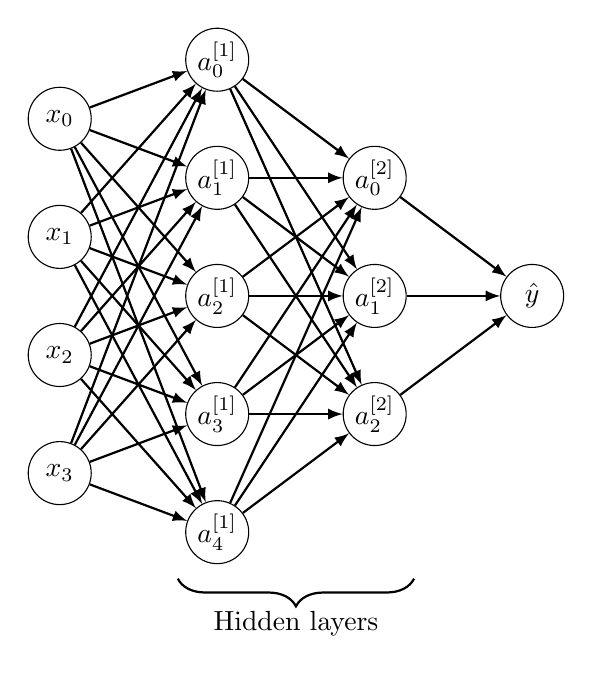
\begin{tikzpicture}[]


\begin{scope}[every node/.style={circle, draw, minimum size=8mm}]
\node (x0) at (0, 0.0) {$x_0$};
\node (x1) at (0, -1.5) {$x_1$};
\node (x2) at (0, -3.0) {$x_2$};
\node (x3) at (0, -4.5) {$x_3$};
\node[inner sep=0pt] (a0) at (2.0, 0.75) {\mySize $a_{0}^{[1]}$};
\node[inner sep=0pt] (a1) at (2.0, -0.75) {\mySize $a_{1}^{[1]}$};
\node[inner sep=0pt] (a2) at (2.0, -2.25) {\mySize $a_{2}^{[1]}$};
\node[inner sep=0pt] (a3) at (2.0, -3.75) {\mySize $a_{3}^{[1]}$};
\node[inner sep=0pt] (a4) at (2.0, -5.25) {\mySize $a_{4}^{[1]}$};
\node[inner sep=0pt] (a5) at (4.0, -0.75) {\mySize $a_{0}^{[2]}$};
\node[inner sep=0pt] (a6) at (4.0, -2.25) {\mySize $a_{1}^{[2]}$};
\node[inner sep=0pt] (a7) at (4.0, -3.75) {\mySize $a_{2}^{[2]}$};
\node[inner sep=0pt] (a8) at (6.0, -2.25) {$\hat{y}$};
\end{scope}
\begin{scope}[-latex, thick]
\draw (x0) -- (a0);
\draw (x1) -- (a0);
\draw (x2) -- (a0);
\draw (x3) -- (a0);
\draw (x0) -- (a1);
\draw (x1) -- (a1);
\draw (x2) -- (a1);
\draw (x3) -- (a1);
\draw (x0) -- (a2);
\draw (x1) -- (a2);
\draw (x2) -- (a2);
\draw (x3) -- (a2);
\draw (x0) -- (a3);
\draw (x1) -- (a3);
\draw (x2) -- (a3);
\draw (x3) -- (a3);
\draw (x0) -- (a4);
\draw (x1) -- (a4);
\draw (x2) -- (a4);
\draw (x3) -- (a4);
\draw (a0) -- (a5);
\draw (a1) -- (a5);
\draw (a2) -- (a5);
\draw (a3) -- (a5);
\draw (a4) -- (a5);
\draw (a0) -- (a6);
\draw (a1) -- (a6);
\draw (a2) -- (a6);
\draw (a3) -- (a6);
\draw (a4) -- (a6);
\draw (a0) -- (a7);
\draw (a1) -- (a7);
\draw (a2) -- (a7);
\draw (a3) -- (a7);
\draw (a4) -- (a7);
\draw (a5) -- (a8);
\draw (a6) -- (a8);
\draw (a7) -- (a8);
\end{scope}

\draw [thick,decorate,decoration={brace,amplitude=10pt,mirror,raise=4pt},yshift=0pt] (1.5,-5.7) -- (4.5,-5.7) node[midway, below, yshift=-12pt] {Hidden layers};


\end{tikzpicture}
\end{document}

